\section{Tutorials 7 (11 IV 2019)}
\subsection*{Büchi-Landweber thm.}
Let $G$ be an $\omega$-regular game, i.e. the winning strategy is $\omega$-regular.
Then, ether of the players has a winning strategy.\\

\noindent
$\langle V, E, v_I, \lambda, L \rangle$\\
$\lambda(v_0...v_n...) \in L$.\\
1) $L$ is regular $\Rightarrow$ $L$ recognized by Deterministic Müller Automaton $\mathcal{A}$.\\
2) $G'$ is a Müller Game created as a product of $(V, E, \lambda) \times \mathcal{A}$.\\
3) Adam/Eve wins in $G'$ $\Rightarrow$ Adam/Eve wins in $G$.

\subsubsection*{Complexities}
\textbf{Problem 1.}\\
\underline{In.} $G = \langle B, L(A) \rangle$ $\leftarrow$ $\omega$-regular game.\\
\underline{Out.} Does Eve win?\\
\begin{itemize}
    \item[a)] $A$ is a deterministic parity automaton.\\
    The upper bound is $NP \cap coNP$, because $G$ is a parity game.
    Algorithm: Reduce $G$ to $G' = G \times A$ parity game, solve $G'$.
    Lower bound: can encode parity games.
    \item[b)] $A$ is a DMA.
    \item[c)] $A$ is a non-deterministic Büchi automaton.\\
    Algorithm: compute DPA $A'$ such that $L(A) = L(A^\prime)$, $|a|^{|a|}$, $[0, 2|a|]$, use (a). This is in EXP.
\end{itemize}

\subsection*{Flow Games}
\begin{figure}[H]
    \centering
    \caption{Example flow game}
    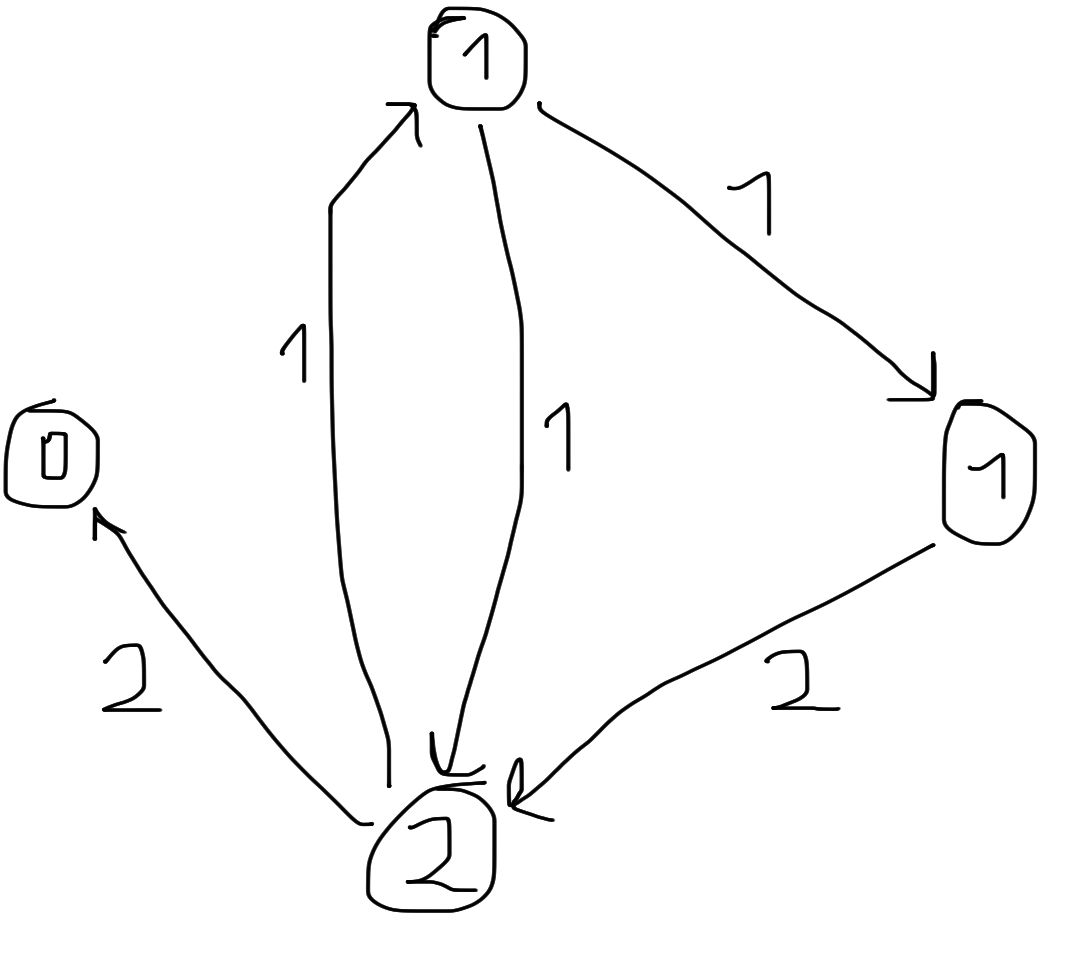
\includegraphics[scale=0.1]{content/graphics/game8.png}
\end{figure}
$G = (V, E, E_{\diamond} \dot\cup E_{\square}, \lambda, e \in E)$.\\
$\lambda\ :\ E \cup V \rightarrow [0, d]$\\
Valid is $\forall_{v} \lambda(v) \leq \underset{(a, v) \in E}{\sum} \lambda(a, v)$.\\
A player $P \in \{\diamond, \square\}$ chooses an edge $e \in E_p$, and flips it.\\
Player $\diamond$ wins if a predefined edge $e$ is flipped.\\
\textbf{Problem 2.} Show that if there is only one player $\diamond$, and every edge can be flipped at most once,
then the game is NP-complete.\\
\underline{In NP:} It is in NP because we can guess the witness in NP and verify in polynomial time.\\
\underline{Complete:} Reduction $3$-SAT\footnote{
    \noindent
    $3$-SAT: Formula $F_1 \land F_2 ... \land F_n$, s.t. $F_i = x_{i_1} \lor x_{i_2} \lor x_{i_3}$ s.t.
    $x_j = y_i$ (or $\lnot y_i$) for $y_1 ... y_k$.
} $\rightarrow$ Game.\\

\noindent
\textbf{Problem 3.} Show that if w allow that an edge is fliped at most once, then the game is APTIME-complete, PSPACE-complete.
